% ---------------------------------------------------
% ----- Introduction of the template
% ----- for Bachelor-, Master thesis and class papers
% ---------------------------------------------------
%  Created by C. Müller-Birn on 2012-08-17, CC-BY-SA 3.0.
%  Last upadte: C. Müller-Birn 2015-11-27 
%  Freie Universität Berlin, Institute of Computer Science, Human Centered Computing. 
%
\chapter{Einleitung}
\label{chap:introduction}

%Im folgenden werden Ihnen Hinweise zur Strukturierung und zum Inhalt des ersten
% Kapitels gegeben.

\section{Thema und Kontext}

%\subsection{Motivation}
%Die Speicherung von Wissen und Daten in digitaler Form ist heute zu einem sehr
%wichtigen Werkzeug geworden, um kollaborativ und global unabhängig von der
% Fachrichtung gemeinsam zu arbeiten. Damit diese Daten in einem Kontext stehen
% und semantisch untereinander und mit anderen Daten verknüpft werden können,
% werden Ontologien entwickelt. In Ontologien wird dann festgelegt, welche Daten wichtig sind und wie sie untereinander in Beziehung stehen. Üblicherweise werden Ontologien für einen bestimmten Bereich oder ein Gebiet erstellt, z.B. eine Tierart oder eine Büchersammlung. Aber auch allgemeiner gefasste Ontologien wurden u.a. im Rahmen der Dublin Core Metadata Initiative  entwickelt. Diese werden konkret dafür benutzt, jegliche Art von Dokumenten und Webressourcen zu beschreiben.\\
%Neben der Speicherung von Wissen finden Techniken und Wissen aus dem Bereichen
%des Semantic Web und der Ontologien in anderen Bereichen Anwendung, allen voran
%Machine und Deep Learning. Einerseits als Anwendungsfall für das Finden von
% Matchings \cite{Doa16} , da es sich gut dafür eignet. Andererseits werden Ontologien für das Speichern gewonnener Informationen verwendet \cite{Pun07} . Damit finden Ontologien in einem aktuell im Fokus stehenden Feld von Wissenschaft und Praxis statt.\\
%Da Ontologien, wie erwähnt, Anwendung in zahlreichen Gebieten finden, gibt es
%Bedarf an Software, mit der auch technisch nicht-versierte Personen arbeiten
% können. \cite{Ber14}

\subsection{Thematische Einordnung}
In der Informatik bezeichnet eine Ontologie je nach Definition „eine
konzeptuelle Formalisierung von Wissensbereichen (Domänen oder Subdomänen)“ \cite{Bie02}  oder auch eine „explizite formale Spezifikation einer gemeinsamen Konzeptualisierung“ \cite{Hes02} . Beide Formulierungen beinhalten, dass etwas formal definiert wird. Die erste beschränkt sich auf individuelle Wissensbereiche, während die zweite Aussage einen Austausch durch eine gemeinsame Konzeptualisierung verschiedener Beteiligter betont. Anwendung finden Ontologien in der Aufbereitung von semantischem Wissen für Datenmengen, indem Konzepte in Strukturen überführt werden. Dadurch wird diesen Datenmengen eine Semantik gegeben. Das ermöglicht es, die Verbindungen und den „Sinn“ auch bei automatischer Verarbeitung dieser Daten zu erhalten bzw. zu berücksichtigen. Insbesondere hilft die Semantik auch dabei, den Kontext von Entitäten in der Ontologie zu erläutern. \cite{Bie02} Dies schafft eine gemeinsame Grundlage, auf der Daten behandelt und betrachtet werden. So arbeiten alle Nutzer, die eine Ontologie verwenden, auch mit demselben Vokabular, was Missverständnisse verringert. Weiterhin müssen in einem Team, welches Ontologien für die Arbeit mit Daten einsetzt, nicht alle Mitglieder vollständiges und tiefgründiges Wissen über die Domäne haben, in der gearbeitet wird.\\
Um die Domäne bzw. den Umfang einer Ontologie zu bestimmen, werden zwei Stufen
definiert. Top Level Ontologien beziehen sich auf Definitionen, die unabhängig von spezifischen Domänen Anwendung finden. \cite{Bie02}  \cite{Hes02}  Ein Beispiel dafür ist der bereits erwähnte Dublin Core für jede Art von Dokumenten. Domain oder Task Ontologien beschäftigen sich mit Begriffe für einen bestimmten Anwendungsbereich. \cite{Bie02}  \cite{Hes02}  Beispielhaft dafür ist die Music Ontology, welche „Informationen mit Bezug zur Musikindustrie“   behandelt.\\
Um Ontologien nicht nur isoliert zu betrachten und da bestimmte Dinge und
Konzepte in mehr als einer Domäne vorzufinden sind, beispielsweise Dokumente als
Ressourcen, bietet es sich an, Ontologien zu matchen. Eine Möglichkeit Ontologien und deren Matching zu beschreiben, ist eine Ontologie mathematisch zu definieren als ein Paar O = (S, A). Dabei ist S die (ontologische) Signatur, die den Wortschatz beschreibt, und A ein Set aus (ontologischen) Axiomen, die die Interpretation des Wortschatzes in der gewünschten Domäne festlegen. Im Rahmen dieser Definition ist ein Matching f: S1 -> S2 eine Verknüpfung der Wortschätze zweier Ontologien O1 = (S1, A1) und O2 = (S2, A2)  unter Beachtung der Struktur der Signaturen und der Interpretationen. Das Matching einer Ontologie ist dann mathematisch gesehen ein Morphismus der Signaturen, so dass gilt A2 |= f(A1). D.h. alle Interpretationen, die die Axiome A2 der Ontologie O2 erfüllen, müssen auch für die übersetzten Axiome f(A1) von Ontologie O1 gelten. \cite{Hoo14}\\
Unter dem Begriff Konzept wird im Bereich der Ontologien nahezu alles verstanden, z.B. Dinge, Gedanken oder Begriffe. \cite{Usc95}  Diese Konzepte dienen dazu, Teile der Realität, Daten oder Strukturen in eben diesen Ontologien abzubilden.

\section{Zielsetzung der Arbeit}
Das Ergebnis dieser Masterarbeit ist eine für technisch nicht versierte Nutzer
gedachte Software, die dazu dient Ontologien zu matchen. Das Hauptaugenmerk soll dabei auf guter Bedienbarkeit liegen.\\
Dabei sollen dem Nutzer Vorschläge für ein Matching unterbreitet werden. Diese
sollen sich anhand eines Algorithmus ergeben. Dieser Algorithmus beinhaltet eine oder mehrere Vorgehensweisen, nach denen Ontologien gematcht werden. Der Nutzer kann dann die vorgeschlagenen Matches akzeptieren, verwerfen und andere hinzufügen.\\
Die Matching-Methoden sollen nicht exklusiv und ausschließlich vorgegeben sein, sondern es muss möglich sein, sie zu verändern. Weiterhin soll es möglich sein, andere Methoden zu verwenden, als die zum Ende der Masterarbeit hin implementierten und auch Methoden, die nach dem Ende der Masterarbeit entwickelt werden, sollen Verwendung finden können, soweit möglich. Daher wird die Architektur der Software modular aufgebaut sein.

\section{Vorgehen bei der Umsetzung}

\subsection{Methodische Umsetzung}
Um gewünschte Software mit der notwendigen Funktionalität umzusetzen, werden eine Reihe an Methoden Anwendung finden. Die schon in der Beschreibung der Software erwähnten Vorschläge deuten bereits an, dass auch Recommender Systeme Einzug in die Software finden werden. Der übliche Fokus von Recommender Systemen auf die Empfehlung von Produkten o.ä. (basierend den Daten von Nutzern) wird allerdings nicht genutzt. Es ist zwar denkbar, die Entscheidungen des oder anderer Nutzer in spätere automatische Matchings einzubeziehen, aber das Augenmerk der Software soll nicht direkt darauf liegen, dem Anwender Matchings zu zeigen, die ihm persönlich gefallen, sondern welche, die sinnvoll sind. Da die Software auch über eine graphische Benutzeroberfläche (GUI) verfügen soll und sich Ontologien und verknüpfte Datenmengen gut als Graph visualisieren lassen, lassen sich auch Techniken aus dem Gebiet der Information Visualization integrieren.

\subsection{Technische Umsetzung}
Aufgrund der großen Möglichkeiten, die moderne Webtechnologien bieten, wird das
Frontend in diesen umgesetzt. Das hat den Vorteil, dass eine Unabhängigkeit des
Betriebssystems bzw. der Nutzungsplattform gegeben ist. Webstandards wurden in
den letzten Jahren erheblich in ihrer Funktionsvielfalt erweitert und über
verschiedene Browser vereinheitlicht. Weiterhin muss neben einem Browser keine
weitere Software installiert werden, sondern das Tool kann sofort genutzt
werden. Die meisten Browser gibt es außerdem für nahezu alle Betriebssysteme,
egal ob auf Desktop/Laptop oder Mobilgeräten wie Smartphones oder Tablets. Damit
werden die Benutzer mit der Technik bedient, die sie selbst verwenden, ohne
eine Laufzeit Umgebung vorauszusetzen, z.B. die Java Runtime Environment für
Java Programme oder eine Python Installation für bestimmte
Betriebssysteme, wo es nicht vorinstalliert ist..\\
Das Backend wird in Python implementiert und dann durch Django eingebettet, um
als Gesamtstück mit dem Frontend zu kommunizieren. Dadurch sind umfangreiche und
rechenintensive Arbeiten möglich. Das ist zwar theoretisch innerhalb von
Browsern möglich, jedoch eher ungewöhnlich und wird in der Regel durch die Dauer
der Operationen von Browsern als unerwünschtes Verhalten gewertet.

%\section{Aufbau der Arbeit}
%\begin{itemize}
%	\item Welche Schritte werden durchlaufen, um die Ziele zu erreichen?
%	\item An dieser Stelle ist beispielsweise eine Grafik hilfreich, um den Aufbau
	% der Arbeit und welche Ergebnisse/Erkenntnisse wo genutzt werden, zu
	% visualisieren.
%	\item Ebenfalls sollten noch Anmerkungen zur Gestaltung der Arbeit gegeben
	% werden, vor allem, da in vielen deutschen Arbeiten englische Fachbegriffe
	% verwendet werden. Ein solcher Text könnte folgendermaßen lauten:
%		\begin{itemize}
%			\item ``Abschließend sind hier noch eine Anmerkungen zur Gestaltung der
			% vorliegenden Arbeit. Für die im Folgenden verwendeten personenbezogene
			% Ausdrücke wurde, um die Lesbarkeit der Arbeit zu erhöhen, die männliche Schreibweise gewählt. Des Weiteren werden eine Reihe von englischen Bezeichnungen verwendet, um einerseits dem interessierten Leser das Studium der häufig vorliegenden englischen Originalliteratur zu erleichtern oder andererseits bestehende Fachbegriffe nicht durch die Übersetzung zu verfälschen. Diese Begriffe sind vom herkömmlichen Text in kursiver Schrift unterschieden.''
%		\end{itemize}
%\end{itemize}

%\begin{figure}[!ht]
	% Mit [!h] wird die Position der Grafik bestimmt. So bedeutet h=here und mit dem "!" (Ausrufezeichen) wird dieser Befehl verstärkt. Weitere Möglichkeiten sind : t=top und b=bottom. Zumeist wird angegeben, in welcher Reihenfolge LaTeX versuchen soll das Bild einzufügen, z.B. [!htb].
%	\centering
%		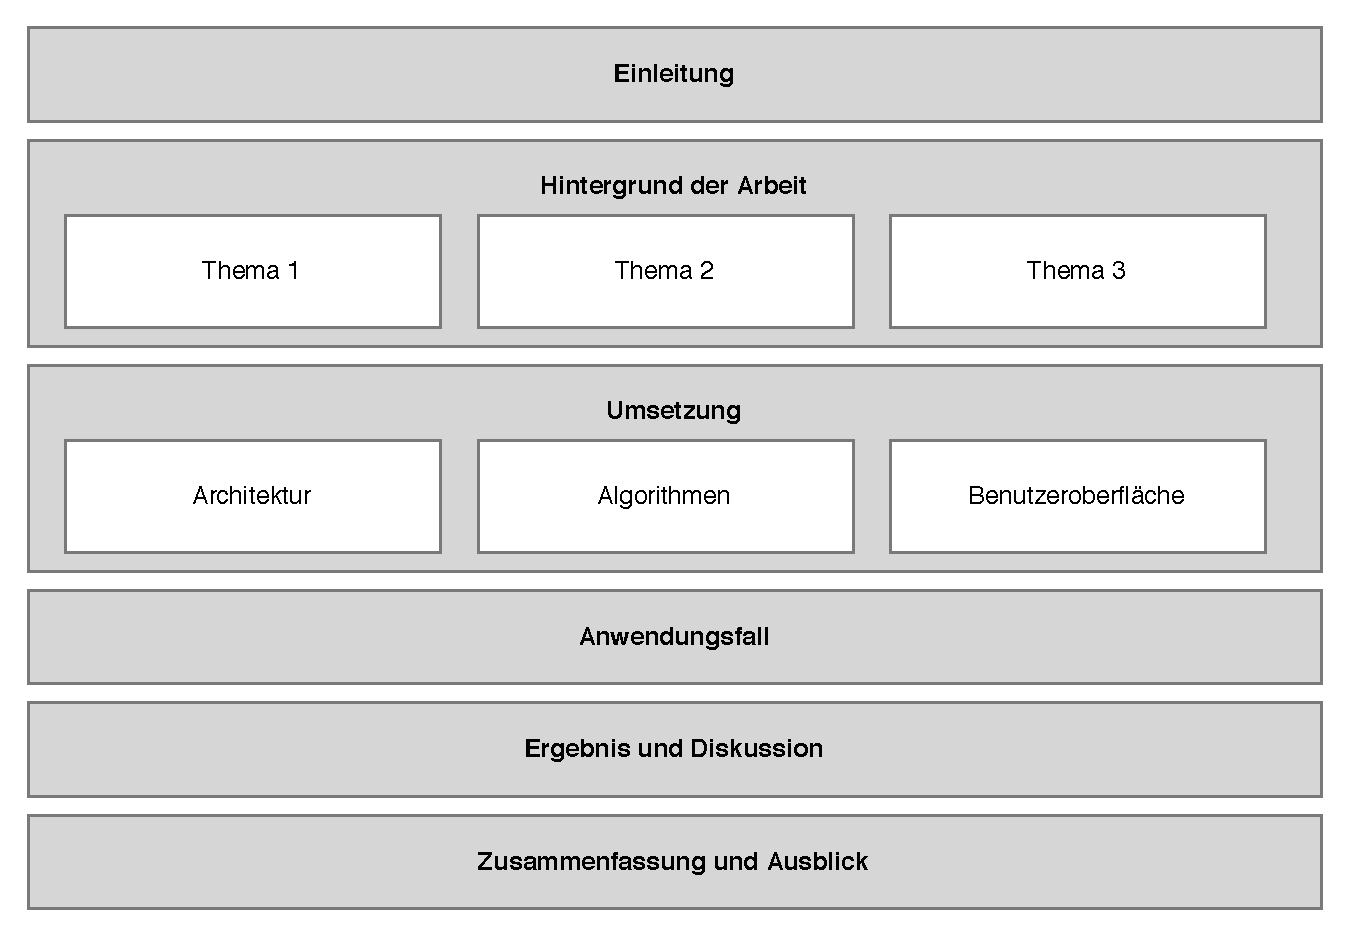
\includegraphics[width=0.95\textwidth]{pics/structure.pdf}
%	\caption[Beispiel einer möglichen Darstellung zum Aufbau der Arbeit]{Beispiel
	% einer möglichen Darstellung zum Aufbau der Arbeit (vgl. Beschreibung Abschnitt  \ref{chap:chapters}).}
	% Mit Hilfe von caption wird die Bildunterschrift erzeugt. Der Text in geschweiften Klammern erscheint im Text, während der Text in eckigen Klammern sich dann empfiehlt, wenn die Beschreibung besonders lang ist, denn diese wird dann im Bildverzeichnis verwendet. Diese Kurzbeschreibung kann auch weggelassen werden. 
%	\label{fig:structurethesis}
%\end{figure}